% Benchmarking in Unity
% https://blogs.unity3d.com/2018/09/25/performance-benchmarking-in-unity-how-to-get-started/
% Maybe try VRWorks https://developer.nvidia.com/vrworks

% Questions to answer in the evaluation chapter:
% \begin{enumerate}
%   \item{How big can the graph be so that it is comfortable visualizing the network?}\\
%   What is comfortable? Number of FPS?
%   How can we scale the graph? By adding nodes and spread them around, by adding more interconnexions?
%   Should the experiment split in several parts? Scaling, filtering, moving around, etc.
%   What is the performance by using Oculus Link and the performance using just the Quest hardware?
%   -We can use the Unity GPU Profiler for Oculus Quest and Go in order to see the performance.\\
%   \href{https://developer.oculus.com/blog/getting-started-w-the-unity-gpu-profiler-for-oculus-quest-and-go/}{See: Getting Started w/ The Unity GPU Profiler for Oculus Quest and Go}
%   \item{How is this way of visualizing the graph better by using VR?}\\
%   We are researchging the technology and the test with actual users is for future work.
%   \item{In what way can the application and the visualization of the graph be improved?}\\
%   Argue in the discussion part.
% \end{enumerate}

% Links
% Profiler panel

GeneNet VR has been developed to explore biological networks that contain genetic information. For this project, we have used two datasets from MIxT \cite{dumeaux_fjukstad_interactions_tumor_blood}, where we applied several VR techniques to build a visualization and interaction system. In this chapter we want to evaluate GeneNet VR, focusing on its scalability and performance. Since we are visualizing networks with genetic information, we want to know if the system that we built can be used for larger sizes of this type of datasets. As part of the evaluation process, we designed a list of questions that we will try to answer along this chapter. The questions are:
\begin{enumerate}
  \item For which interactions do we achieve the recommended FPS (72) when scaling the network?
  \item What characteristics of the network influence the scalability?
  \item What is the performance by using a PC with Oculus Link and the performance using just the Quest hardware?
  % \item Bonus: how will “beautifications” influence scalability?
  \item How do users perceive the interaction of the network?
\end{enumerate}

Question one is based on the Oculus' performance guidelines\cite{oculus_performance_baselines}, that say that an application should meet the following:
\begin{itemize}
  \item 72 FPS for Oculus Quest (required by Oculus).
  \item 50-100 draw calls per frame.
  \item 50,000-100,000 triangles or vertices per frame.
\end{itemize}

We will evaluate the performance for the interactions we use most for the visualization of the networks. These are: translation of the network, scaling of the network and node selection (including the line rendering for the relationships).

As for the second question, we want to know what characteristics influence the scalability of the system. Some parts of the application will have more impact on the performance than others. To keep it simple, we will evaluate the impact in the performance done by the following elements, that are the most important for the visualization: number of nodes,  number of lines and number of clusters. However, since the cluster algorithm is applied when initializing the network, we will just focus on the number of nodes and the number of lines.

We will also evaluate the performance of the application being run in the Oculus Quest hardware and compare it with the performance in the PC. The hardware of the Oculus Quest is not as powerful as the one of the machine that was used for the development. We would like to know if the performance in the Oculus Headset is good enough for the visualization of MIxT.

Finally, we want to know how the users perceive the interaction and visualization of the network. We will evaluate this with a qualitative method with a demo of the application using the MIxT datasets and also an interview.

\section{Experimentation plan}
An experimentation plan was designed to ensure that the experiments are consistent and that they can be reproduced several times in order to get realistic measurements. We take into consideration the following aspects for our experiments:
\begin{enumerate}
  \item Scalability for different interactions.
  \item Network characteristics.
  \item Bottlenecks.
  \item User study.
  \item Hardware and software specification.
\end{enumerate}

As we mentioned before, we will evaluate the performance of the system when we translate, scale and select nodes in the network. We will focus on the number of nodes and lines that the network has to have an idea of how the network scales. While studying the performance we will also see if there are bottlenecks and what is causing them. We will describe in Table \ref{tab:network-elements} the elements of the system that can more impact in the scalability.

\begin{table}[h!]
\centering
\begin{tabular}{l p{9cm}}
\textbf{Element} & \textbf{Description} \\
Clusters & The algorithm used to create the clusters is run in the initialization of the system, before everything renders. This can be time consuming because it involves many operations to process the text files (they have several thousands of lines). However this is only called at the beginning and not after the system is initialized. \\
Nodes   & Represented as 2D squares in the space, they consist of 2 triangles. They are always showing in the scene and they position change while scaling and translating the network.  \\
Lines & They represent relationships between the nodes. Everytime a node is selected, line objects are added to the scene. They are 2-dimensional and consist of 2 triangles. Depending on the node we might need to render several hundreds of these lines in the scene. \\
\end{tabular}
\caption{Elements of the network that have influence in the scalability.}
\label{tab:network-elements}
\end{table}

We have designed a series of experiments that can be reapeated several times. We ran each experiment 4 times and calculate the average in order to get realistic results. We also created a benchmark in Unity using C\# where we reproduce the interactions that we want to evaluate. The experiments are coded in the benchmark using scripts so that we can always reproduce them. For the networks translation and network scale we use mathematical functions to translate the network around the scene and to scale the network up and down. For the node selection we have chosen a set of nodes.

As for the hardware specification, we ran the experiments in a machine with Windows 10. In Table \ref{tab:machine-specs} we can see the hardware specification for the machine. The GPU is also specified in Table \ref{tab:gpu-specs}. The hardware specification of the Oculus Quest is shown in Table \ref{tab:oculus-specs}.

\begin{table}[h!]
\centering
\begin{tabular}{ll}
\multicolumn{2}{c}{Machine specification}                        \\
Processor   & Intel(R) Xeon(R) CPU E3-1275 v6 @ 2.80GHz 3.79 GHz \\
RAM memory  & 64.0 GB                                            \\
System type & 64-bit Operating System
\end{tabular}
\caption{Machine specification.}
\label{tab:machine-specs}
\end{table}

\begin{table}[h!]
\centering
\begin{tabular}{ll}
\multicolumn{2}{c}{GPU specification} \\
Adapter type   & NVIDIA GeForce GTX 1080 Ti \\
Chip Type  &  GeForce GTX 1080 Ti \\
DAC Type & Integrated RAMDAC \\
Available memory & 45025 MB
\end{tabular}
\caption{GPU specification.}
\label{tab:gpu-specs}
\end{table}

\begin{table}[h!]
\centering
\begin{tabular}{ll}
\multicolumn{2}{c}{Oculus Quest specifications} \\
Panel Type   & Dual OLED 1600x1440 \\
Supported Refresh Rate  &  72Hz \\
Tracking & Inside out, 6DOF \\
CPU & Qualcomm® Snapdragon 835 \\
GPU & Qualcomm® Adreno™ 540 GPU \\
Memory & 4GB total
\end{tabular}
\caption{Oculus Quest specifications.}
\label{tab:oculus-specs}
\end{table}

The experiments were run in Unity, the same software that we used for the development. We used the version 2018.4.10f1 of Unity for the whole project and experimentation. In Unity we used the OpenGL graphic API.

% @TODO Write about how scalability was tested.
In order to find bottlenecks, we used a profiling tool in Unity. A profiler is used to get an overview of the performance of the application. We used the built-in profiler in Unity. This gave us information about per-fram CPU  performance metrics. In addition, Unity also provides some metric information that we can be displayed in the Unity editor. We got information about the number of vertices in the scene, triangles, frames per second, etc.

\section{Performance evaluation}
We will explain in this section the experiments to evaluate the performance. We will also show the results that we obtained and discuss them. As we mentioned before, we will focus on the performance for several actions that the user usually does when exploring the networks. These are translation of the network, scale up or down the network and select nodes in the network as well as render the lines for the relationships. All the experimens are run 4 times and we show the averages.

We ran all the experiments on the PC and we used the blood dataset from MIxT. We chose this dataset because it is bigger than the biopsy one. We also ran each experiment for different sizes of the blood dataset: the whole dataset (2693 nodes), half size of the dataset (1346 nodes) and a third part (897 nodes). In order to analyse the performance, we obtained the deltaTime for each frame. In Unity, this variable privides the time between the current and the previous frame. Once we obtain all the times for all the frames that the experiments last, we extract make the following calculations: the average of all the times of the frames, the 0.25\% worst of all the frames and the 0.1\% worst of all the frames.

% Draw calls: https://medium.com/@toncijukic/draw-calls-in-a-nutshell-597330a85381
% Basically a draw call contains all the information telling GPU about textures, states, shaders, rendering objects, buffers, etc. encapsulated as CPU work that prepares drawing resources for the graphics card. Converting state vectors (all the information mentioned before) to hardware commands for the GPU is very “expensive” for the CPU and API complexity becomes API overhead that does not help.

\subsection{Performance when translating the network}
In this experiment, we evaluate the performance when translating the network. To translate the network around in the scene, we have used a sine function in the y axis and a constant function in the z axis. For every frame we update the y and z position of the network object, creating a wave motion. We obtain the delta time for every frame during a total of 700 frames (starting from frame number 501 until frame 1200). In Table \ref{tab:experiment_moving} we can see the results obtained in the experiment for all the network sizes and with the averages.

\begin{table}[h!]
\centering
\begin{tabular}{llll}
Dataset size & 1\% average low & 0.25\% average low & Average \\
size & 12.174 & 20.111 & 6.553 \\
size/2 & 12.791 & 21.996 & 6.498 \\
size/3 & 13.516 & 23.28 & 6.495 \\
\end{tabular}
\caption{Performance results when translating the network.}
\label{tab:experiment_moving}
\end{table}

The average for all the sizes is quite similar. We can also see that the average time is slightly lower when the network is smaller. For the 1\% column, we calculate the average for the 7 frames with highest times. For the 0.25\% column, we do something similar; we show the time of the frame with the worst time. As we can see, the times for these percentages are actually higher when the network is smaller, something that we didn't expect. We would have expected that the time was lower when the number of nodes was lower as well. However, for the total averages, this tendency meets our expectations.

\subsection{Performance when scaling the network}
In this experiment, we evaluate the performance when scaling up and down the network. We use a sine function as well. we update the size of the network object for every frame and since we use a sinus function, the network scales up an down several times. We obtain the delta time for every frame during a total of 700 frames, as well as in the translation performance experiment. See Table \ref{tab:experiment_scale} for the results obtained.

\begin{table}[h!]
\centering
\begin{tabular}{llll}
Dataset size & 1\% average low & 0.25\% average low & Average \\
size & 13.418 & 22.816 & 6.505 \\
size/2 & 12.685 & 22.607 & 6.485 \\
size/3 & 13.631 & 23.015 & 6.494 \\
\end{tabular}
\caption{Performance of scale the network.}
\label{tab:experiment_scale}
\end{table}

The results from this experiment are similar to the ones obtained in the previous one about the translation of the network, but we find some differences. The average time for all the nodes (3rd column) is slightly different, the time for size/3 is higher than size/2, somthing that we would have expected the opposite. All the results for the size/2 are lower than for size/3.

\subsection{Performance when selecting nodes}
In this experiment we want to evaluate the performance when selecting nodes. When a node is selected in GeneNet VR, several things are done during this process. First, an algorithm finds the node that the user is trying to select. Second, two text objects are updated with the new names of the gene node. Thrid, the relationships from that node are rendered in the scene. There are many things going on during this process and we evaluate the performance for the entire pipeline.

As for the experiment design, we took into consideration the number of the relationships (lines) that had to be drawn in the scene. In the blood dataset, a node can have between 1 and 1607 edges. We wanted to have a balanced number of this for our experiment, so we decided to select several nodes that cover this range.

In Figure \ref{fig:edges_nodes_blood} we show a scatter plot where the X axis represents the the number of edges in ascendent order and the Y axis represents the number of nodes that have that number of edges. As we can see, most of the nodes have less than 100 edges. For instance, there are 117 nodes that have 2 edges, and 231 nodes that have just 1 edge. This suppose already the 12,92\% of all the nodes in the dataset. However there also a few nodes that have several hundred of lines. Because it was a bit hard to make a balanced selection, we just selected several nodes from the range 1 to 1607. The nodes that we select during the experiment are the following (in parenthesis the number of edges that they have): TGFBR3 (1), EPSTI1(11), SMNDC1(90), HNRNPH3(290), ANGEL2(586), ACTR6(756), ARGLU1(1607).

% Example scatter plot https://timodenk.com/blog/latex-plot-snippets/screen-shot-2017-02-18-at-15-10-07/
% https://tex.stackexchange.com/questions/390161/drawing-3d-points-from-external-file
\begin{figure}[h!]
  \centering
  \begin{minipage}{.8\textwidth}
  \begin{tikzpicture}
    \begin{axis}
    [ xlabel=Number of edges,
    ylabel=Number of nodes,
    xmin=0,xmax=1610,
    ymin=0,ymax=240,
    ]
    \addplot[only marks,mark=asterisk,color=rred, style={thick}] file{data/bloodEdges.dat};
    \end{axis}

    \end{tikzpicture}
  \end{minipage}
\caption{Scatter plot showing a distribution of the number of edges in the blood dataset. The X axis shows the number of edges and the Y axes shows the number of nodes that have that number of edges in the blood dataset.}
\label{fig:edges_nodes_blood}
\end{figure}

In the experiment, we select the nodes that we mentioned before. We select one node every 100 frames, starting from the TGFBR3 node and following the order from the list. We calculate the averages after all the nodes have been selected. We also have a total of 700 frames, like in the previous experiments. In Figure \ref{tab:experiment_select} we can see the results.

\begin{table}[h!]
\centering
\begin{tabular}{llll}
Dataset size & 1\% average low & 0.25\% average low & Average \\
size & 65.569 & 100 & 8.711 \\
size/2 & 56.389 & 100 & 8.638 \\
size/3 & 56.385 & 100 & 8.583 \\
\end{tabular}
\caption{Performance of select node.}
\label{tab:experiment_select}
\end{table}

The average delta time is a bit higher than the ones in the translation and scaling experiments (around 2 milliseconds more). In the low percentages we can see a big difference though. For the 0.25\%, it's always 100ms. And for the 1\% everage low, it's 65ms for the whole size and 56ms for size/2 and size/3. We can see that the node selection can have much more impact in the performance than the translation and scale of the network.

\subsection{Performance discussion}
We can see from the results, that the number of nodes in the dataset doesn't have that much impact in the performance. It would be interesting to analyse the performance wiht datasets that have more than 2693 nodes. For instance with 5000 and 10000 nodes, but for our project, we have just focused on the datasets MIxT, and the blood dataset is the biggest one. For a future work, it would be interesting to analyse larger datasets to see if the number of nodes could influence more in the performance.

\begin{figure}[h!]
\centering
\begin{tikzpicture}
    \begin{axis}[
        width  = 0.8*\textwidth,
        height = 8cm,
        major x tick style = transparent,
        ybar=2*\pgflinewidth,
        bar width=14pt,
        ymajorgrids = true,
        ylabel = {Delta Time (ms)},
        symbolic x coords={Translate,Scale,Select Node},
        xtick = data,
        scaled y ticks = false,
        enlarge x limits=0.25,
        ymin=0,
        legend cell align=left,
        legend style={
                at={(1,1.05)},
                anchor=south east,
                column sep=1ex
        },
        extra y ticks = 0.4,
        extra y tick labels={},
        extra y tick style={grid=major,major grid style={thick,draw=black}}
        ]
        \addplot[style={bblue,fill=bblue,mark=none}]
            coordinates {(Translate, 12.174) (Scale,13.418) (Select Node,65.569)};
            coordinates {(Translate, 20.111) (Scale,22.816) (Select Node,100)};

        \addplot[style={rred,fill=rred,mark=none}]
             coordinates {(Translate,12.791) (Scale,12.685) (Select Node,56.389)};

        \addplot[style={ggreen,fill=ggreen,mark=none}]
             coordinates {(Translate,13.516) (Scale,13.631) (Select Node,56.385)};

        \legend{Size,Size/2,Size/3}
        \addlegendimage{my legend}
    \end{axis}
\end{tikzpicture}
\caption{Bar graph showing a summary of the performance results for the 1\% lowest average (7 frames with worst performance or higher times).}
\label{fig:performance_bar}
\end{figure}

In general, the performance is good for the experiments that we ran. Having an average of 7-8 milliseconds for all the frames means that we meet the 72 FPS that the Oculus' performance guidelines suggest. However, for the node selection, we have seen that the performance can be a lot worse than for the other interactions, see Figure \ref{fig:performance_bar} for a summary of the results. In this bar graph we can see a summary of the 1\% worst time for the different interactions. We can see that the time for the node selection interaction is much higher.

One important observation is that in the experiment we just select 7 nodes, one every 100 frame. However, when we use GeneNete VR, it's easy to select many nodes in just a few frames. This is because the select node function is run for every frame when we trigger the action for it, and if we point at a region where there are many nodes together, it will be easy to select several of them in a short period of time. Another point to take into account is that not all the nodes have the same number of edges to render. It would be interesting to know if the number of edges could decrease the performance as well. We will analyse in the following section if the selection of nodes and the number of edges could have more impact in the performance and scalability of the network.

\section{Scalability evaluation}
As we saw in the performance experiment for selecting the nodes, the time to render the frames can be very high. This could have influence in the quality of the application and generate some unconformity in the user's experience. It could happen that the application freezes for some milliseconds and that the application doesn't run smoothly when selecting the nodes. In this section we evaluate the performance when selecting the nodes and rendering the edges for the nodes. This will also help us study the scalability of the application so that it can be used for larger datasets.

We would like to know if the number of edges that we need to render in the scene can decrease the performance. We designed an experiment where we test the delta time (the time that a frame takes to render) for different amount of edges to render. In Figure \ref{fig:edges_nodes_blood} we showed the distribution between the number of edges and the number of nodes that have that amount of edges. We used this data and created a new dataset where we have a node from every "edge category" and then we selected each of the nodes and calculated the delta time. To put it simple we try to render the edges for each of the possible number of edges that we can find in the blood dataset and calculate the time for each of them.

In Figure \ref{fig:scalability_edges_blood} we can see the results for this experiment. In our benchmark we run the select node action for each of the nodes from the dataset that we created for this. We select a new node in each frame. We show the results using an scatter plot. The X axis represents the number of edges to render. The Y axis represents the total time that it took to render that amount of edges.

We would have expected that when there are more edges to render, more time it would be needed for that. However, that is not as clear in the experiments results. We can see that when there are less than 200 edges, many of the times are less than 20ms. Nevertheless, some nodes that have less than 200 edges take more than 40 or even 50 ms to render. On the right side of the plot we can see that some nodes with several hundreds of edges take more than 60 ms to render, but in some cases they take less than 20 ms. This is not very consisten and we conclude here that the number of edges might influnce in the performance, but we can see that there are many other things that influence the performance as well. Unity is a complex game engine, and there are many things going on when we run the experiments.

\begin{figure}[h!]
  \centering
  \begin{minipage}{.8\textwidth}
  \begin{tikzpicture}
    \begin{axis}
    [ xlabel=Number of edges,
    ylabel=Time (ms),
    xmin=0,xmax=1610,
    ymin=0,ymax=100,
    ]
    \addplot[only marks,mark=asterisk,color=rred, style={thick}] file{data/scalabilityBlood.dat};
    \end{axis}

    \end{tikzpicture}
  \end{minipage}
\caption{Scatter plot showing the relation between the number of edges to render and the time that it takes to render for the blood dataset.}
\label{fig:scalability_edges_blood}
\end{figure}

After running this experiment we ran the profiler from Unity to see what could be the cause for taking so much time when selecting some nodes. We profiled the selection of the node ARGLU1(1607), which has the maximum number of edges. In Figure \ref{fig:profiler}, we can see an screenshot of the profiler in Unity. In the profiler window we can see a graph where the Y axis shows the amount of time that each frame took to render. we are selecting a frame in the middle, where we can see a spike (althugh it's a bit hard to see because of the selection bar). This frame corresponds with the selection of the node. It took 121.23ms to render. In the Overview window we can see a list of functions that are called during this frame. Also there are several columns and the the total column indicates the percentage of the time that a particular function took. As can see in the screenshot, we don't get much information about where the proble could be. But we can see that 65.4\% of the total time comes from the BehaviourUpdate function.

\begin{figure}
    \centering%
    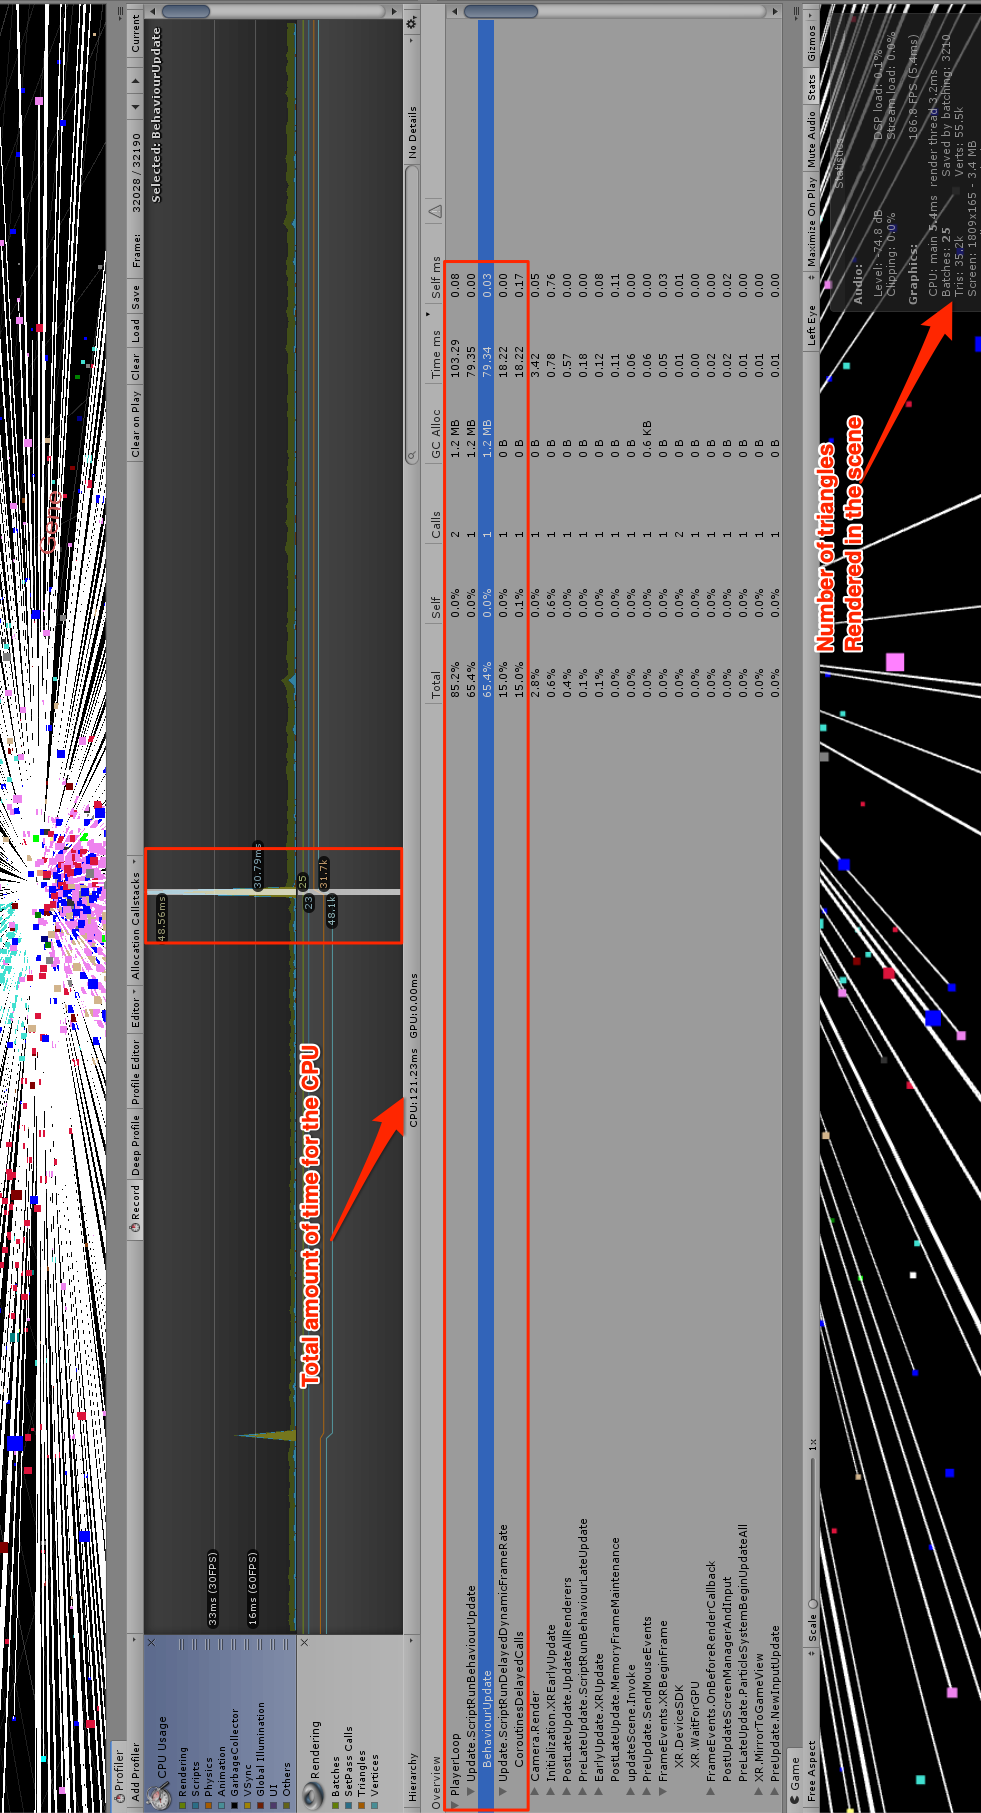
\includegraphics[width=0.9\textwidth]{profiler}
    \caption{Profiling the selection of the node ARGLU1(1607), which has the highest number of edges. We study what is the cause for the high amount of time that this takes to render.}
    \label{fig:profiler}
\end{figure}%

We get also some other metric information from this screenshot (see the region far below and the small black grey square with the Statistics title), like the number of triangles that the scene is rendering. This is the selection of the node with the highest number of edges and there are a total of 35.2k verteces, which is inside of the Oculus' performance guidelines.

% \begin{figure}[h!]
%   \centering
%   \begin{minipage}{.9\textwidth}
%   \begin{tikzpicture}
%     \begin{axis}
%     [ xlabel=Number of edges,
%     ylabel=Time (ms),
%     xmin=0,xmax=430,
%     ymin=0,ymax=100,
%     ]
%     \addplot[only marks, mark=asterisk, color=rred, style={thick}] file{data/scalabilityBiopsy.dat};
%     \end{axis}
%
%     \end{tikzpicture}
%   \end{minipage}
% \caption{Scatter plot showing the relation between the number of edges to render and the time that it takes to render for the biopsy dataset.}
% \label{fig:scalability_edges_biopsy}
% \end{figure}

\section{Oculus Quest vs Computer}
We developed the application in a PC and tested it in Oculus Quest, an standalone headset. We did the testing using a USB C cable that connects the headset to the PC. However when we run the application in this way, we use the PC's hardware. The previous experiments were also run in the PC. We want to evaluate in this section, if the performance in the Oculus Quest is good enough when running GeneNet VR. The hardware for the Oculus Quest is not as good as for the machine, so we expect that the performance in the Oculus Quest is goin to be worse.

\begin{figure}[h!]
  \centering
  \begin{minipage}{.8\textwidth}
  \begin{tikzpicture}
    \begin{axis}
    [ xlabel=Frame number,
    ylabel=Time (ms),
    xmin=301,xmax=370,
    ymin=0,ymax=100,
    legend pos=north west,
    ]
    \addplot[color=rred, style={thick}] file{data/headset.dat};
    \addlegendentry{Oculus Quest}
    \addplot[color=bblue, style={thick}] file{data/pc.dat};
    \addlegendentry{PC}
    \end{axis}

    \end{tikzpicture}
  \end{minipage}
\caption{Performance running the application in a machine vs on Oculus Quest.}
\label{fig:pc_vs_oculus}
\end{figure}

We designed an experiment that we could run in the PC and in the Oculus Quest to measure the performance for each of the machines. In the experiment we run several things at the same time. We used a combination of the three performance experiments that we explained before and use them together for this experiment. For a short period of time we translate the network, scale it and select several nodes, everything at the same time. The experiment lasts for 70 frames; it starts in frame 300 and ends in frame 370.

In Figure \ref{fig:pc_vs_oculus}, we can see the results from the experiment, represented with a graph. The X axis represents the frame number (like a timeline). The Y axis represents the amount of time that a particular frame took to render in milliseconds. We can see that the performance for the Oculus Quest is a bit worse than for the PC; however, the difference is not very big. We can also see some peaks in the graph. This is due to the select node action. We select 7 nodes during the experiment. A new node is selected every 10 frames. The node selection starts in frame 300 with a node that doesn't have many edges and the last node of the experimen (in frame 360 has many nodes). Each new node selected has more edges that the previous one. We can see this refleted in the graph; every 10 frames there is a new picks, starting from frame 330, and this pick is higher. We can say that the number of edges has an impact with the performance.

\section{Demo and interview}
One of the questions that we asked ourselves during the evaluation process was about how the users perceive the interactions with the networks. In order to evaluate this we made a qualitative questionnaire for users to answer when testing the application. Unfortunately, due to the Covid-19 situtation\cite{covid_19}, we were not able to carry out the questionnaire with many people. It wasn't possible to test GeneNet VR with people on a single Oculus Quest device without avoiding the social distancing rules. We estimated to have around 10 participants with knowdledge in bioinformatics to. With this number of participants, we could have made some statistics and obtained feedback for future improvement. However, due to the situation, we just tested it with one person.

Questions related to the locomotion of the VR application:
\begin{itemize}
  \item Can you teleport yourself to other parts of the scene? Is it easy to telepor yourself to the place that you want to teleport to?
  \item Can you teleport yourself to a spot in the scene a face that direction that you want? Is it easy to do this?
  \item Can you snap rotate to visualize the scene from other angles? Is it easy to do this?
\end{itemize}

Questions related to interaction with the network:
\begin{itemize}
  \item Can you select a node? Is it easy to select the node that you want with the laser pointer?
  \item Can you select a node that is far away? Is it easy to precisely that node that you want to select?
  \item Can you translate the network to other position?
  \item Can you scale the network?
  \item Can you morph the network from one dataset to another?
\end{itemize}

% The following questionnaire is divided in four sections; a general section about VR headsets, a section about comfortability exploring the network using GeneNet VR, a section about the different actions in GeneNet VR and finally a section about feedback.
%
% To complete the questionnaire, the teste has to indicate the level of agreement or disagreement with each of the  statements, mark yes or no when it is asked and in the feedback section reply the questions with constructive feedback if possible.\\

% TODO Interview questions

% Questionnaire section 1: VR headsets.
% \begin{enumerate}
%   \item Have you ever used a VR headset before?\\
%   Yes / No
%
%   \item Have you ever used a Oculus Quest headset before?\\
%   Yes / No
%
%   \item I feel comfortable using a VR headset.\\
%   Strongly agree / Agree / Neutral / Disagree / Strongly Disagree
%
%   \item I feel comfortable using the Oculus Quest headset.\\
%   Strongly agree / Agree / Neutral / Disagree / Strongly Disagree\\
% \end{enumerate}
%
% Questionnaire section 2: Comfortability exploring a biological network with GeneNet VR.
% \begin{enumerate}
%   \item I feel comfortable moving around the virtual environment using the teleport functionality.\\
%   Strongly agree / Agree / Neutral / Disagree / Strongly Disagree
%
%   \item I feel comfortable rotating to any direction.\\
%   Strongly agree / Agree / Neutral / Disagree / Strongly Disagree
%
%   \item I feel comfortable visualizing the network by moving my head.\\
%   Strongly agree / Agree / Neutral / Disagree / Strongly Disagree
%
%   \item I feel comfortable selecting the nodes to visualize the relationships.\\
%   Strongly agree / Agree / Neutral / Disagree / Strongly Disagree
%
%   \item I feel comfortable moving the network to the position that I want.\\
%   Strongly agree / Agree / Neutral / Disagree / Strongly Disagree
%
%   \item I feel comfortable scaling the network.\\
%   Strongly agree / Agree / Neutral / Disagree / Strongly Disagree
%
%   \item I feel comfortable using the UI menu to filter the data from the network.\\
%   Strongly agree / Agree / Neutral / Disagree / Strongly Disagree\\
% \end{enumerate}
%
% Questionnaire section 3: Performing different actions in GeneNet VR to explore the biological network.
% \begin{enumerate}
%   \item It is intuitive to manipulate the network using the controllers.\\
%   Strongly agree / Agree / Neutral / Disagree / Strongly Disagree
%
%   \item The different actions in the controllers are easy to learn and remember.\\
%   Strongly agree / Agree / Neutral / Disagree / Strongly Disagree
%
%   \item I can move the network to any position that I want.\\
%   Strongly agree / Agree / Neutral / Disagree / Strongly Disagree
%
%   \item I can scale the network to any size that I want.\\
%   Strongly agree / Agree / Neutral / Disagree / Strongly Disagree
%
%   \item I can select any node that I want.\\
%   Strongly agree / Agree / Neutral / Disagree / Strongly Disagree
%
%   \item I can easily visualize the relationships of any node.\\
%   Strongly agree / Agree / Neutral / Disagree / Strongly Disagree
%
%   \item I can easily filter the data by using the UI menu.\\
%   Strongly agree / Agree / Neutral / Disagree / Strongly Disagree\\
% \end{enumerate}
%
% Questionnaire section 4: Feedback.
% \begin{enumerate}
%   \item Did you experience any difficulties exploring the biological network? If so, indicate which ones.\\
%   Yes / No
%
%   \item Is there anything that could be improved for the visualization of biological data in GeneNet VR? If so, write your suggestions.\\
%   Yes / No
%
%   \item Write any feedback and comments that you have about the exploration of biological networks with GeneNet VR.
% \end{enumerate}
